\section{Algoritmo construtivo}

A construção prioriza clientes com maiores demandas. Para o cliente escolhido, avaliam-se as posições viáveis nas rotas. O custo incremental de uma inserção é
\[
\Delta=C(R^{p,v})-C(R).
\]
Os candidatos formam a RCL definida por
\begin{equation}
\Delta \leq c_{min}+\alpha(c_{max}-c_{min}),
\end{equation}
e uma posição é sorteada nessa lista.

Assim, $\alpha=0$ admite apenas o melhor incremento, $\alpha=1$ aceita todos os candidatos viáveis e valores intermediários equilibram guloseima e aleatoriedade. Os custos são recalculados após cada inserção. Quando não há candidato viável, uma busca limitada por backtracking distribui os clientes restantes.

\begin{figure}[H]
\centering
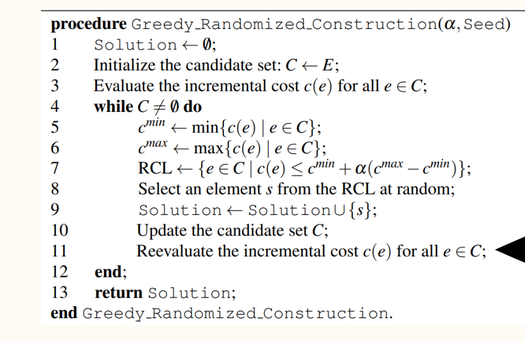
\includegraphics[width=0.72\textwidth]{imagens/pseudo-codigo-construcao.png}
\caption{Pseudocódigo da construção gulosa aleatorizada.}
\label{fig:pseudoconstrucao}
\end{figure}
